\documentclass[12pt, letterpaper]{article}
\usepackage{fontspec}
\setmainfont{Palatino Linotype}
\usepackage[parfill]{parskip}
\usepackage{fullpage}
\usepackage[none]{hyphenat}
\usepackage{graphicx}


\begin{document}


\title{The Application of DevOps in Campus Area Networks}
\author{Shivam Singh}
\date{\today}
\maketitle


\begin{center}

A Proposal Presented to\\ 
The Department of the Information Science and Technology\\
College of Science Technology and Applied Arts of Trinidad and Tobago 

\vspace{1cm}

In (Partial) Fulfillment\\
of the Requirements for the Degree\\
Bachelor of Science

\end{center}

\newpage
\tableofcontents

\newpage

\section{Executive Summary}

\begin{center}
\textit{This document serves as a proposal to adopt a DevOps approach to managing the network infrastructure for the College of Science, Technology and Applied Arts of Trinidad and Tobago.}
\end{center}

	\subsection{Why is this solution necessary ?}
	\subsection{What this proposal does not cover and why it is not covered ?}
This solution does not include the implementation of the following elements.
\begin{itemize}
\item Wireless Access
\item Data Center Configurations
\item Voice and Collaboration
\end{itemize}

The reason for not including these topics within the proposal is because it would require 
which would far exceed the purpose of this proposal. This is not a fully proposed solution but rather a stepping stone and guideline towards change in

	
	
\newpage
\section{Introduction}

	\subsection{Client Background}
The client COSTAATT is a public tertiary institution in Trinidad and Tobago that offers programs in the areas of Information Technology, Business and Nursing, just to name a few.
	
\medskip

The solution proposed can be applied to all types of organizations with large scale networks as it is aimed towards addressing the management of a large topology with limited human resources. The reason COSTAATT is an ideal candidate for this solution is because of their vast amount of networks and communication equipment that span multiple campuses across Trinidad and Tobago. 
	
	\subsection{Problem}
Many critical services such as file sharing, active directory and email services which was originally on premise is now being hosted in cloud based platforms or being migrated to decentralized infrastructure such as remote data centres. This means that high availability fault tolerant networks have become a necessity in order to ensure consistent access to these core services. There is room for improvement with regards 

	\subsection{Cause of the Problem}
The traditional methods of managing the network has led to longer turnaround times with regards to troubleshooting issues, and scalability when making changes in the network to accommodate new devices or applications. This causes a halt in productivity as well as growth in the organization when they attempt to integrate new services 

	\subsection{Aim}
Implement a DevOps solution that enhances the management of COSTAATT's network which will improve system uptime and increased productivity for the organization. The solution contributes to productivity because automating repeatable or time consuming tasks will allow IT operations to concentrate on projects geared towards optimizing performance.

\newpage

	\subsection{Evaluation}
The delivery of the following components will determine the success of this project.

\medskip

Build a network topology that is up to standards with regards to security and guidelines of Campus Area Networks. I will be relying on the NSA’s Network Infrastructure Security Guide as well as Cisco’s guide on implementing Campus Area Networks. 

\medskip

The devices must be communicating successfully with one another. We can use simple ping test in order to determine this. 

\medskip

The Ansible framework must be able to communicate with all devices that support SSH and I should be able to push configuration changes to all devices successfully. Ansible has built in features that indicate if you have successfully pushed configurations to a device. 

\medskip

Hypothetical scenarios will be introduced into the environment such as device or link failures and we will utilize the tools that we implemented to quickly recover. Failure to recover within an acceptable time frame will determine if the solution is fault tolerant. We want to recover within minutes. Examples of mass configuration changes will be carried out to test the efficiency of using Ansible. 

\newpage

\begin{figure}
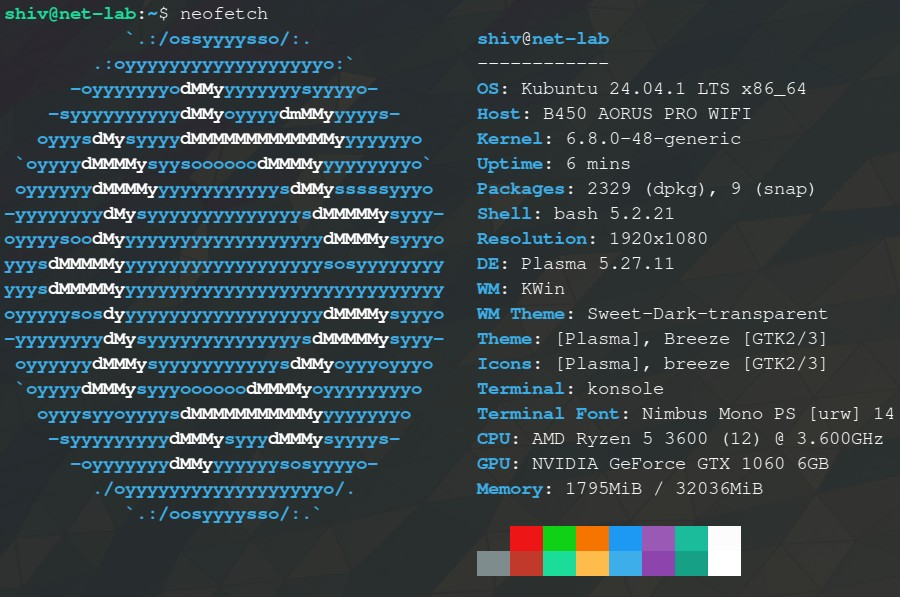
\includegraphics[scale=0.65]{neofetch_Output.jpg}
\end{figure}





\end{document}